\begin{minipage}{0.25\textwidth}
	\centering
	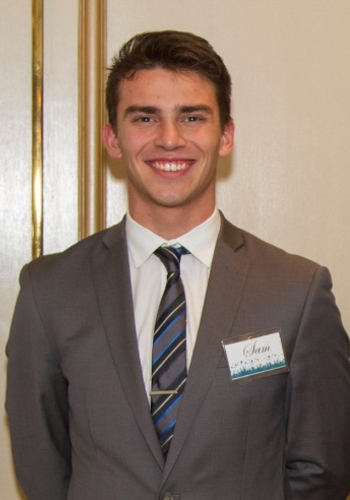
\includegraphics[width=\textwidth]{fmt-dotson.jpg}
\end{minipage}
\begin{minipage}{0.73\textwidth}
	$\textbf{General Co-Chair - Sam Dotson}$\\
Sam graduated with a B.S. in Physics from UIUC in 2019. He attended his first ANS student conference in April 2019 and was so inspired by his experience that he decided to pursue graduate work in nuclear engineering rather than physics. Now he does research on machine learning applications and computational reactor physics with Dr. Kathryn Huff in the ARFC group. Hosting a student conference that will inspire others the way he was inspired is one of his top priorities this year. He has experience planning activities for student organizations such as Guidance for Physics Students (GPS) and has experience fundraising for the College of Lake County (CLC). He helped set a record amount of donations at the 2016 CLC Foundation Gala, where he was an invited speaker and volunteer. He will be attending the ANS National conference in November 2019, as well as the ANS Student Conference 2020 at North Carolina State University.
\end{minipage}

\begin{minipage}{0.25\textwidth}
	\centering
	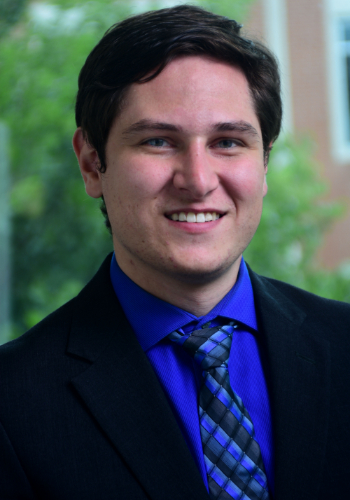
\includegraphics[width=\textwidth]{fmt-mettler.jpg}
\end{minipage}
\begin{minipage}{0.73\textwidth}
	$\textbf{Technical Co-Chair - Jeremy Mettler}$\\
Jeremy graduated with a B.S. in Nuclear, Plasma, and Radiological Engineering from UIUC in 2018, and is now attending as a 2nd-year graduate student studying plasma science under Dr. David Ruzic. He has been heavily involved in the UIUC student chapter of ANS since his freshman year, serving on the executive board for three years as External Vice President and President. Jeremy has attended the past five ANS Student Conferences, which serve as an inspiration for his involvement in this proposal process. He is dedicated to making sure that future generations of students are able to have the same amazing experiences through ANS as he had, especially at the ANS Student Conference. Outside of ANS, he has held a summer internship at Oak Ridge National Lab, and is currently focusing his research towards combined laser-plasma systems for materials processing.
\end{minipage}

\begin{minipage}{0.25\textwidth}
	\centering
	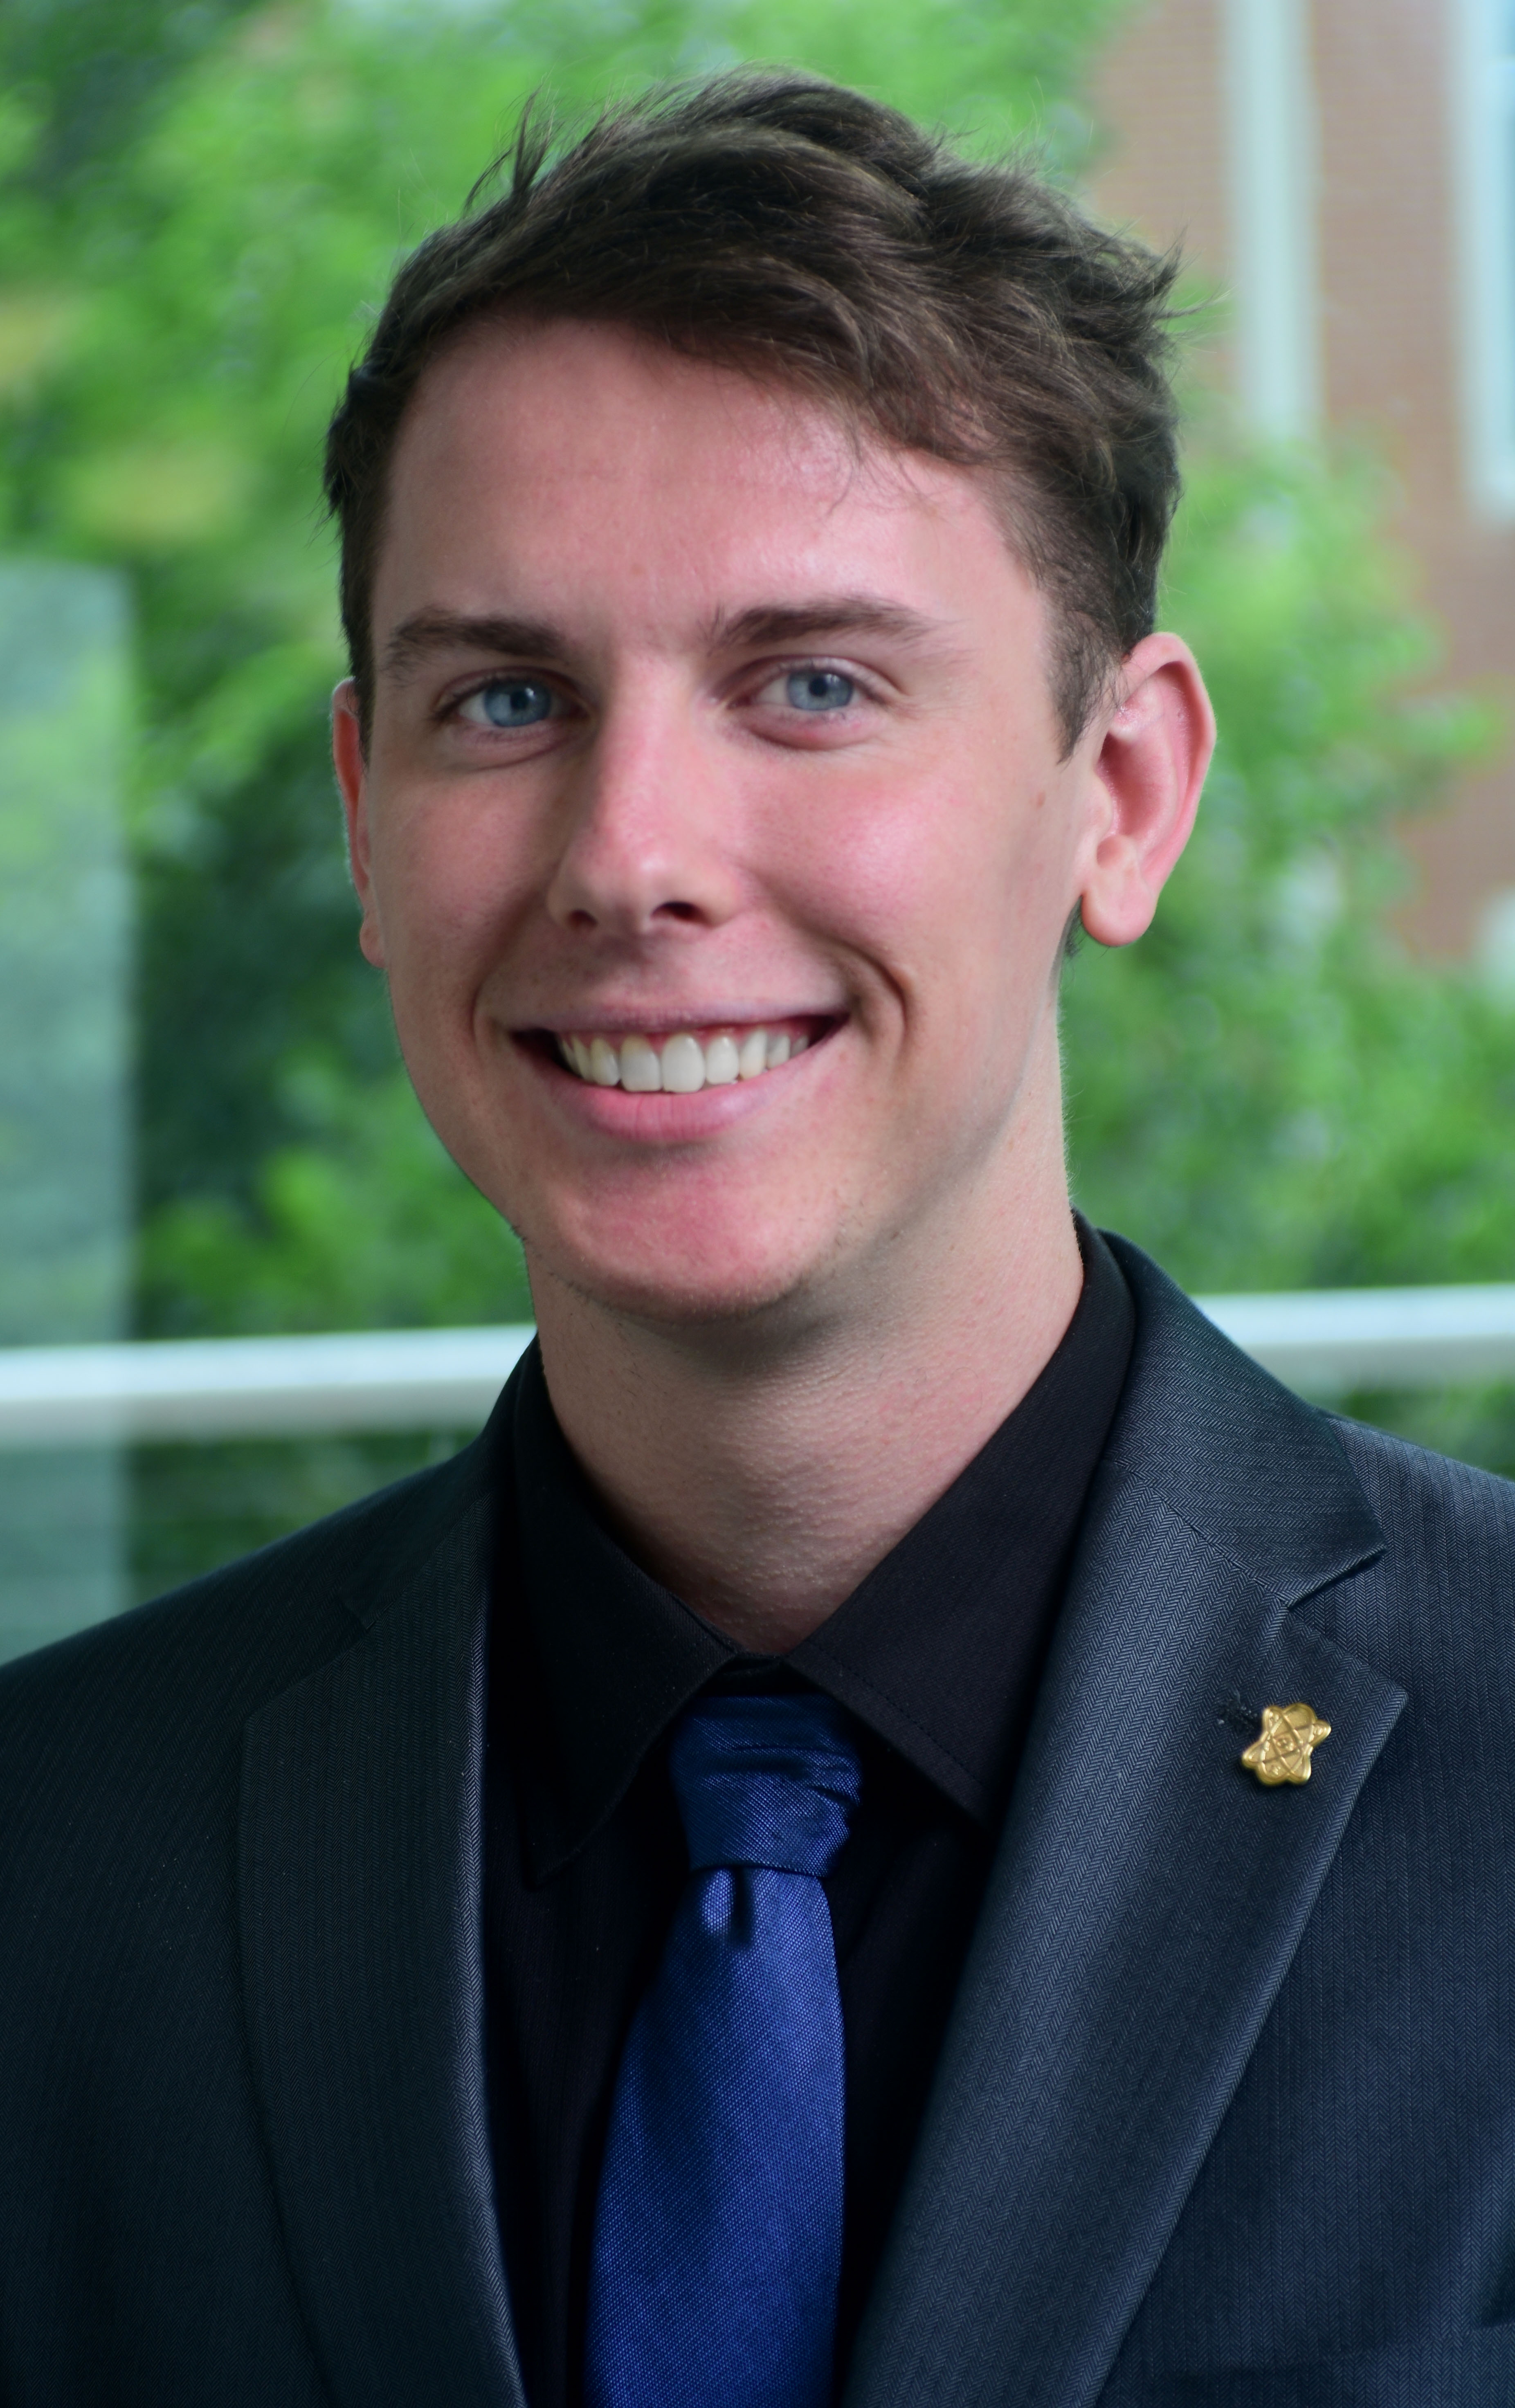
\includegraphics[width=\textwidth]{ncreid2.jpg}
\end{minipage}
\begin{minipage}{0.73\textwidth}
$\textbf{Diversity Co-Chair - Nathan Reid}$\\
	Nate graduated with a B.S. in Nuclear, Plasma, and Radiological Engineering from UIUC in 2016. He is a 4th-year Ph.D. student in the field of fusion and plasma science and engineering under Prof. Jean Paul Allain. Nate is currently conducting his thesis research at Oak Ridge National Laboratory, where he has spent the last three summers working in the nuclear structural materials group under the mentorship of Dr. Lauren Garrison. He will return the UIUC in December 2019. Nate has attended four of the last five ANS Student Conferences and was a student paper competition finalist at the TOFE embedded topical of the 2018 ANS Winter Meeting. Nate has been recognized by the ANS-UIUC for his outstanding graduate service in the last year, and served as the Women in Nuclear UIUC chapter Vice President. He was part of the executive team that received the national student chapter excellence award at the 2019 Women in Nuclear national conference, of which he was awarded a student sponsorship to attend. Nate is ecstatic about working alongside his ANS student section as Diversity Co-Chair and setting goals to bring inclusion to the conference.
\end{minipage}

\begin{minipage}{0.25\textwidth}
	\centering
	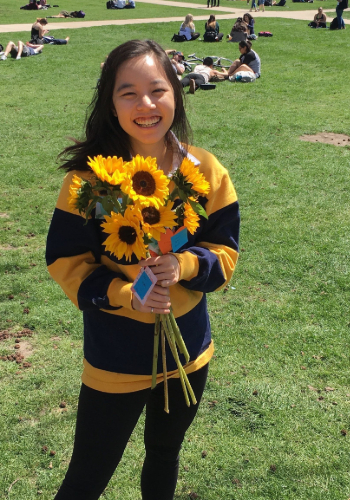
\includegraphics[width=\textwidth]{fmt-chee.jpg}
\end{minipage}
\begin{minipage}{0.73\textwidth}
$\textbf{Technical Subcommittee Chair - Gwendolyn Chee}$\\
	Gwen is a third year graduate student studying fuel cycles for advanced reactor designs with Dr. Kathryn Huff in the ARFC group. Last summer she had an internship at Argonne National Laboratory where she worked on sensitivity analysis of the nuclear fuel complex. She also serves as the president of the UIUC chapter of Women In Nuclear (WIN). Under her leadership, WIN-UIUC was honored with the Best Student Chapter award at the WIN National Meeting in 2019. She has also been involved with ANS and attended the 2018 ANS Student Conference in Florida and will be attending the upcoming ANS Student Conference at NC State in 2020.
\end{minipage}

\begin{minipage}{0.25\textwidth}
	\centering
	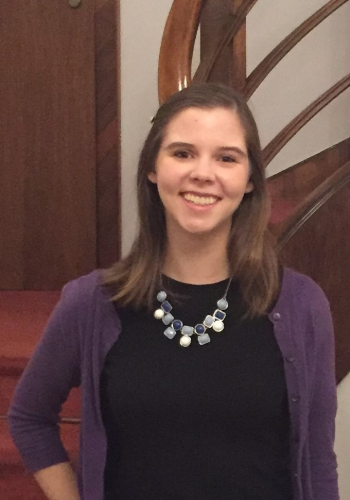
\includegraphics[width=\textwidth]{fmt-gaughan.JPG}
\end{minipage}
\begin{minipage}{0.73\textwidth}
$\textbf{Logistics Chair - Natalie Gaughan}$\\
	Natalie earned her B.S. in Nuclear Engineering from the University of Wisconsin-Madison in 2017. She has completed two summer internships at Argonne National Laboratory where she worked with various neutronics codes. Natalie then spent a year in Vienna as an intern at the International Atomic Energy Agency, where she helped organize and evaluate nuclear data for medical isotope production. She is now a graduate student at UIUC intending to research radiological science and nuclear medicine. As an undergraduate, Natalie attended two ANS student conferences which played a huge role in obtaining internships and inspired her decision to attend graduate school. Natalie knows firsthand how the ANS student conferences can be influential in students’ education and career development, and would love to help younger students experience the same benefits. She will also be attending the upcoming ANS student conference in 2020 at NC State.
\end{minipage}

\begin{minipage}{0.25\textwidth}
	\centering
	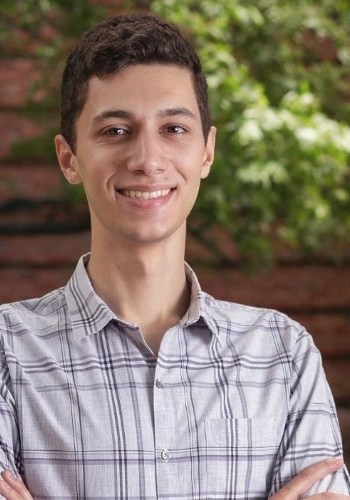
\includegraphics[width=\textwidth]{fmt-stahl.jpg}
\end{minipage}
\begin{minipage}{0.73\textwidth}
	$\textbf{Financial Chair - Jack Stahl}$\\
Jack graduated with a B.S. in Nuclear, Plasma, and Radiological Engineering from UIUC in 2019, and is now a first-year graduate student studying plasma engineering under Dr. David Ruzic. He has been involved in the UIUC student chapter of ANS since his sophomore year and has attended two student conferences. Previously, Jack has spent a summer as an intern at ASML. Jack hopes to help host a student conference that will bolster younger student involvement in ANS.
\end{minipage}

% \vspace{1cm}
\clearpage
\textbf{Financial Subcommittee}\\

\begin{minipage}{0.25\textwidth}
	\centering
	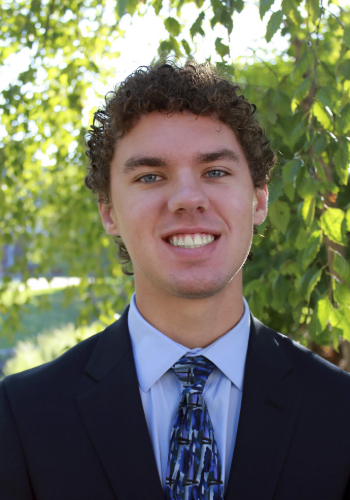
\includegraphics[width=\textwidth]{fmt-shehee.jpg}
\end{minipage}
\begin{minipage}{0.73\textwidth}
	$\textbf{Sponsorship Coordinator - James Shehee}$\\
Jimmy is a junior undergraduate student in UIUC's Nuclear, Plasma, and Radiological Engineering department, with a concentration in power, safety, and the environment. Jimmy has been an active member of the University's ANS student chapter since his freshman year, has held the positions of Secretary and External Vice President, and was chosen to receive the chapter's Undergraduate Outstanding Service Award in the spring of 2019. Jimmy was first introduced to the nuclear industry through the Nuclear Science Merit Badge in Boy Scouts, and he is excited about any opportunity to create similar experiences for students and the public. Outside of ANS, Jimmy is also the President of the Illini Venturing Crew. In the summer of 2019, Jimmy interned at Exelon's Quad Cities Generating Station, and will be returning for another summer in 2020. He is excited to attend his first ANS Student Conference in March 2020 at North Carolina State University.
\end{minipage}

\begin{minipage}{0.25\textwidth}
	\centering
	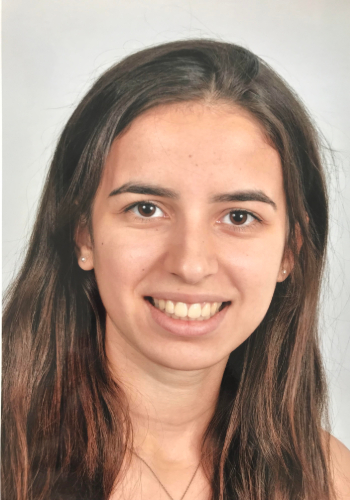
\includegraphics[width=\textwidth]{fmt-dinari.jpg}
\end{minipage}
\begin{minipage}{0.73\textwidth}
	$\textbf{Registration Coordinator - Jasmine Dinari}$\\
Jasmine is a freshman studying Nuclear, Plasma, and Radiological Engineering at UIUC, as well as minors in French and Physics. She is starting research with Dr. Andruczyk, who is currently at the head of the HIDRA project. Powering the world through nuclear is one of her main interests, and she later hopes to participate in nuclear fusion research. The ANS Student Conference is an  amazing opportunity to share her interests in nuclear science. She gained organizational and leadership experience through various extracurriculars in high school and currently serves as the Professional Development Chair for the UIUC student chapter of Women in Nuclear. She plans on attending the 2020 ANS Student Conference at NC State.
\end{minipage}

\vspace{1cm}
\textbf{Technical Subcommittee}\\

\begin{minipage}{0.25\textwidth}
	\centering
	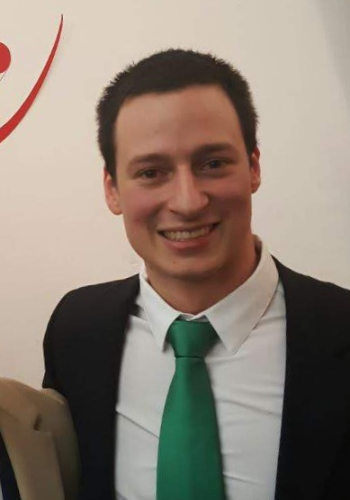
\includegraphics[width=\textwidth]{fmt-fairhurst.jpg}
\end{minipage}
\begin{minipage}{0.73\textwidth}
	$\textbf{Workshops Coordinator - Roberto Fairhurst}$\\
Roberto graduated with a B.S. in Nuclear Engineering from Instituto Balseiro (Argentina) April 2018. He is now a 2nd-year graduate student at UIUC. He does research on computational multi-physics solvers applied to advanced reactors as part of the Advanced Reactors and Fuel Cycle group under the supervision of Dr. Kathryn Huff. He got experience in the organization of conferences during the planning and development of a technical workshop (TWOFCS19) that took place at UIUC in June 2019. His motivation for hosting a student conference is his passion for Nuclear Energy and his desire to transmit this passion to other students. He believes hosting the student conference at UIUC will help the field grow and thrive. This is also an opportunity to meet other people working in the field, share life experiences, and develop a stronger network.
\end{minipage}

\begin{minipage}{0.25\textwidth}
	\centering
	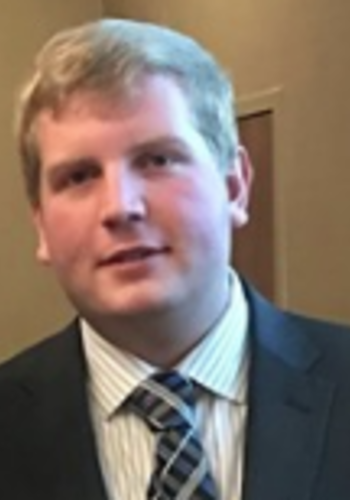
\includegraphics[width=\textwidth]{fmt-jeckell.png}
\end{minipage}
\begin{minipage}{0.73\textwidth}
$\textbf{Sessions Coordinator - Zachary Jeckell}$\\
	Zachary graduated with a B.S. in Nuclear, Plasma, and Radiological Engineering from UIUC in 2018 and is now a second year graduate student studying plasma engineering under Dr. David Ruzic. He has presented his research at two previous student conferences  and realized that he wanted to help bring this prestigious event to the University of Illinois. He strongly believes that the group of students at UIUC are capable of such a feat and that the University would make an excellent location for the conference because of its stellar program and wonderful faculty. He plans to attend the next ANS student conference at NC State to present research on chemical vapor deposition using atmospheric pressure plasma.
\end{minipage}

\begin{minipage}{0.25\textwidth}
	\centering
	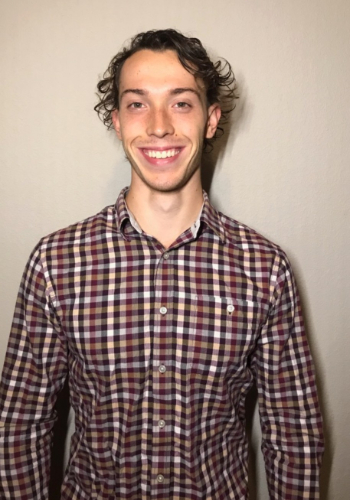
\includegraphics[width=\textwidth]{fmt-golba.jpg}
\end{minipage}
\begin{minipage}{0.73\textwidth}
$\textbf{Career Fair Coordinator - Grzegorz Golba}$\\
	Grzegorz Golba is a sophomore pursuing a B.S. in Nuclear Engineering with a physics minor in the plasma and fusion science concentration. He is now studying material interactions with plasma under Dr. Daniel Andruczyk. Grzegorz attended the 2019 ANS Student Conference in Virginia, reaffirmed his desire to study of nuclear science. He seeks new opportunities to engage with the nuclear science community and is excited for the possibilities of hosting a student conference at UIUC.
\end{minipage}

\vspace{1cm}
\textbf{Non-Technical Subcommittee}\\

\begin{minipage}{0.25\textwidth}
	\centering
	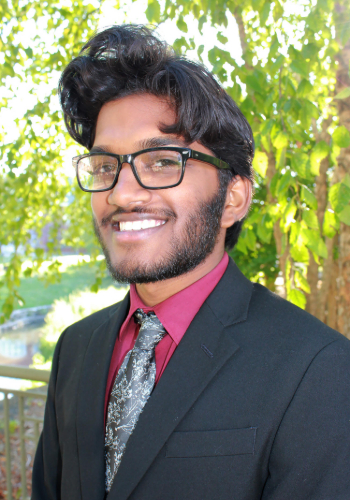
\includegraphics[width=\textwidth]{fmt-dilan.jpg}
\end{minipage}
\begin{minipage}{0.73\textwidth}
	$\textbf{Program Coordinator - Dilan Kurukulasuriya}$\\
Dilan Kurukulasuriay is a sophomore pursuing a B.S. in Nuclear, Plasma, and Radiological Engineering, along with a minor in Physics and Mathematics. He has been active in ANS at UIUC since the start of his freshman year, and he currently serves as the Outreach Chair on the Executive Board. Dilan has worked at the Center for Plasma-Material Interactions lab since the start of his freshman year on HIDRA, and he stayed on campus over the summer to continue to do so. Dilan attended the 2019 ANS Student Conference and it was the highlight of his freshman year of college. He is interested in fusion science research, specifically the materials interaction aspect. He also plans on attending the upcoming student conference at NC State in 2020.
\end{minipage}

\begin{minipage}{0.25\textwidth}
	\centering
	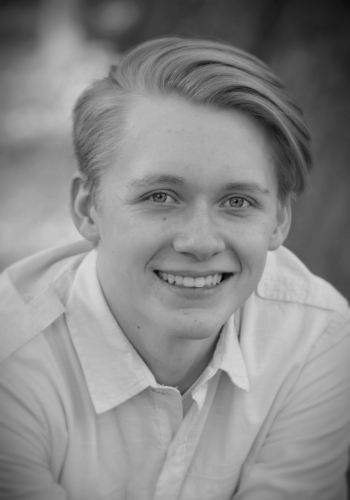
\includegraphics[width=\textwidth]{fmt-davis.jpg}
\end{minipage}
\begin{minipage}{0.73\textwidth}
$\textbf{Hotels and Transportation Coordinator - Gavin Davis}$\\
	Gavin is currently pursuing a B.S. in Nuclear, Plasma, and Radiological Engineering from UIUC and plans to graduate in 2022. He has been involved with the ANS-UIUC since his freshman year and has dedicated his time to outreach events and increasing public awareness of nuclear science and nuclear energy. He has accomplished this through events such as UIUC's Engineering Open House. It was an event he enjoyed as a kid and hopes to help other children develop an interest in nuclear sciences. He also returns to his high school to talk about his experience at UIUC. He looks forward to learning more about nuclear fission technology and to make advancements in nuclear science and in the nuclear energy sector as a whole. He looks forward to attending the student conference at NC State in 2020.
\end{minipage}

\begin{minipage}{0.25\textwidth}
	\centering
	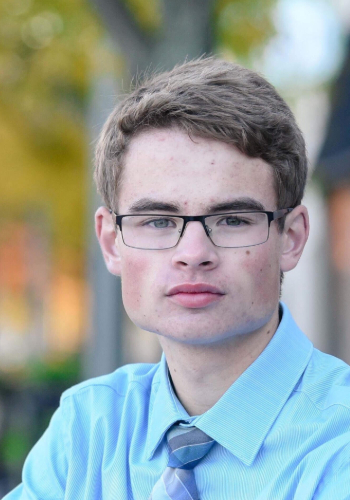
\includegraphics[width=\textwidth]{fmt-moran.jpg}
\end{minipage}
\begin{minipage}{0.73\textwidth}
	$\textbf{Hospitality and Catering Coordinator - Brady Moran}$\\
Brady a freshman in the Nuclear, Plasma, and Radiological Engineering program in the Plasma concentration. He is looking forward to putting his time and efforts toward ANS events throughout his years at UIUC. Last year, Brady planned a large tasting event, the Taste of Sauk Valley, which boasted 550 attendees, $\$$15,000 in revenue, and required him to coordinate 12 restaurants and various subcommittees. He is confident that this experience will help him make the Student Conference a great success. He will be attending the 2020 conference at NC State.
\end{minipage}

\begin{minipage}{0.25\textwidth}
	\centering
	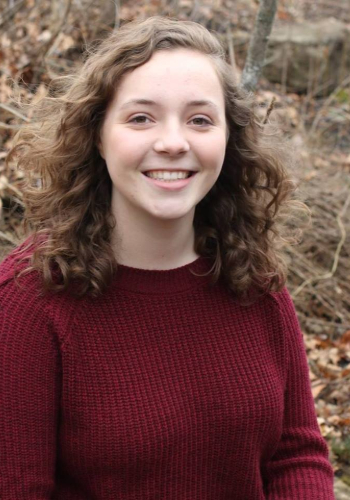
\includegraphics[width=\textwidth]{fmt-balla.jpg}
\end{minipage}
\begin{minipage}{0.73\textwidth}
	$\textbf{Tours Coordinator - Anna Balla}$\\
Anna is a junior in NPRE with a planned concentration in the power, safety, and the environment. She became interested in nuclear engineering after taking a general education class with an NPRE professor and learning about how effective nuclear power is at reducing carbon emissions. Anna is a teaching assistant for two classes in the NPRE department and is also very involved with the Women in Nuclear chapter at Illinois. In her spare time, she enjoys going to concerts, playing volleyball, and wishing she knew how to juggle.
\end{minipage}

\begin{minipage}{0.25\textwidth}
	\centering
	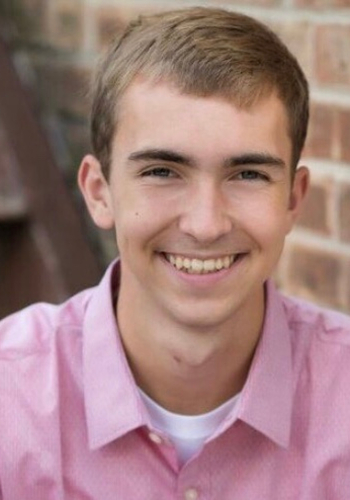
\includegraphics[width=\textwidth]{fmt-ryan.jpg}
\end{minipage}
\begin{minipage}{0.73\textwidth}
$\textbf{Media Coordinator - Nathan Ryan}$\\
	Nathan is pursuing a B.S. in Physics from UIUC. He graduated in the top five of his high school class, while holding down a part time managerial position and running a research project at Argonne National Laboratory concurrent with his Sophomore through Senior years of Secondary Education. His first experience with Nuclear Physics was at the National Superconducting Cyclotron Laboratory where he worked with grad students on rare Cadmium isotopes. He has experience with building appealing website pages, as well as social media communications. He believes that an online presence for this event will supplement the success of an already great set of programs and individuals involved. He is excited to attend the upcoming ANS Student Conference at NC State in 2020.
\end{minipage}
